% -*- latex -*-
%%%%%%%%%%%%%%%%%%%%%%%%%%%%%%%%%%%%%%%%%%%%%%%%%%%%%%%%%%%%%%%%
%%%%%%%%%%%%%%%%%%%%%%%%%%%%%%%%%%%%%%%%%%%%%%%%%%%%%%%%%%%%%%%%
%%%%
%%%% This text file is part of the source of 
%%%% `Parallel Programming in MPI and OpenMP'
%%%% by Victor Eijkhout, copyright 2012-2020
%%%%
%%%% mpi-collective.tex : driver file for the collectives chapter
%%%%
%%%%%%%%%%%%%%%%%%%%%%%%%%%%%%%%%%%%%%%%%%%%%%%%%%%%%%%%%%%%%%%%
%%%%%%%%%%%%%%%%%%%%%%%%%%%%%%%%%%%%%%%%%%%%%%%%%%%%%%%%%%%%%%%%

A certain class of MPI routines are called `collective', or more correctly:
`collective on a communicator'.
This means that if process one in that communicator calls that routine,
they all need to call that routine.
In this chapter we will discuss collective routines
that are about combining the data on all processes
in that communicator,
but there are also operations such as opening a shared file
that are collective, which will be discussed in a later chapter.

\Level 0 {Working with global information}
\label{sec:collective}

If all processes have individual data, for instance the result
of a local computation, you may want to bring that information
together, for instance to find the maximal computed value
or the sum of all values. Conversely, sometimes one processor has
information that needs to be shared with all.
For this sort of operation, MPI
has \indextermdef{collectives}.

There are various cases, illustrated in figure~\ref{fig:collectives},
\begin{figure}[ht]
  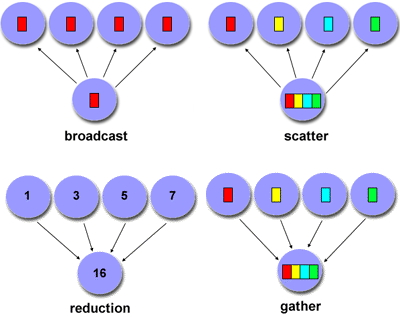
\includegraphics[scale=.8]{collective_comm}  
  \caption{The four most common collectives}
  \label{fig:collectives}
\end{figure}
which you can (sort of) motivate by considering some classroom activities:
\begin{itemize}
\item The teacher tells the class when the exam will be. This is a
  \indextermdef{broadcast}: the same item of information goes to everyone.
\item After the exam, the teacher performs a \indextermdef{gather}
  operation to collect the invidivual exams.
\item On the other hand, when the teacher computes the average grade,
  each student has an individual number, but these are now combined to
  compute a single number. This is a \indextermdef{reduction}.
\item Now the teacher has a list of grades and gives each student their
  grade. This is a \indextermdef{scatter} operation, where one process
  has multiple data items, and gives a different one to all the other
  processes.
\end{itemize}

This story is a little different from what happens with MPI
processes, because these are more symmetric; the process doing the
reducing and broadcasting is no different from the others.
Any process can function as the \indexterm{root process} in such a
collective.

\begin{exercise}
  \label{ex:collective-cases}
  How would you realize the following scenarios with MPI collectives?
  \begin{itemize}
  \item Let each process compute a random number. You want to print the
    maximum of these numbers to your screen.
  \item Each process computes a random number again. Now you want to
    scale these numbers by their maximum. 
  \item Let each process compute a random number. You want to print on what processor the
    maximum value is computed. 
  \end{itemize}
\end{exercise}

\Level 1 {Practical use of collectives}

Collectives are quite common in scientific applications. For instance,
if one process reads data from disc or the commandline, it can use a
broadcast or a gather to get the information to other
processes. Likewise, at the end of a program run, a~gather or
reduction can be used to collect summary information about the program
run.

However, a more common scenario is 
that the result of a collective is needed on all processes.

Consider the computation of the \indexterm{standard deviation}:
\[ \sigma = \sqrt{\frac1{N-1} \sum_i^N (x_i-\mu)^2 }
\qquad\hbox{where}\qquad \mu = \frac{\sum_i^Nx_i}N
\]
and assume that every process stores just one~$x_i$ value.
\begin{enumerate}
\item The calculation of the average~$\mu$ is a reduction, since all
  the distributed values need to be added.
\item Now every
  process needs to compute~$x_i-\mu$ for its value~$x_i$, so $\mu$~is
  needed everywhere. You can compute this by doing a reduction followed
  by a broadcast, but it is better to use a so-called
  \indexterm{allreduce} operation, which does the reduction and leaves
  the result on all processors.
\item The calculation of $\sum_i(x_i-\mu)$ is another sum of
  distributed data, so we need another reduction operation. Depending
  on whether each process needs to know~$\sigma$, we can again use an
  allreduce.
\end{enumerate}

As another examples,
if $x,y$ are distributed vector objects, and you want to compute
\[ y- (x^ty)x \]
which is part of the Gramm-Schmidt algorithm; see~\HPSCref{app:gram-schmidt}.
Again you need to use an allreduce to reduce the inner product value on all processors. 
\begin{lstlisting}
// compute local value
localvalue = innerproduct( x[ localpart], y[ localpart ] );
// compute inner product on the every process
AllReduce( localvalue, reducedvalue );
\end{lstlisting}

\Level 1 {Synchronization}

Collectives are operations that involve all processes in a
communicator. %%(See section~\ref{sec:collectiveslist} for an informal listing.)
A~collective is a
single call, and it blocks on all processors,
meaning that a process calling a collective cannot proceed
until the other processes have similarly called the collective.

That does not mean that
all processors exit the call at the same time: because of
implementational details and network
latency they need not be synchronized in their execution.
However, semantically we can say that
a~process can not finish
a collective until every other process has at least started the collective.

In addition to these collective operations, there are operations that
are said to be `collective on their communicator', but which do not
involve data movement. Collective then means that all processors must
call this routine; not to do so is an error that will 
manifest itself in `hanging' code. One such example is
\indexmpishow{MPI_File_open}.

\Level 1 {Collectives in MPI}

We will now explain the MPI collectives in the following order.
\begin{itemize}
\item[Allreduce] We use the allreduce as an introduction to the
  concepts behind collectives; section~\ref{sec:allreduce}. As
  explained above, this routines serves many practical scenarios.
\item[Broadcast and reduce] We then introduce the concept of a root
  in the reduce (section~\ref{sec:reduce-root}) and broadcast
  (section~\ref{sec:bcast}) collectives.
\item[Gather and scatter] The gather/scatter collectives deal with
  more than a single data item.
\end{itemize}

There are more collectives or variants on the above.
\begin{itemize}
\item If you want to gather or scatter information, but the contribution
  of each processor is of a different size, there are `variable' collectives;
  they have a~\n{v} in the name (section~\ref{sec:v-collective}).
\item Sometimes you want a reduction with partial results, where each processor
  computes the sum (or other operation) on the values of lower-numbered processors.
  For this, you use a \indexterm{scan} collective (section~\ref{sec:scan}).
\item If every processor needs to broadcast to every other, you use an
  \indexterm{all-to-all} operation (section~\ref{sec:alltoall}).
\item A barrier is an operation that makes all processes wait until every
  process has reached the barrier (section~\ref{sec:barrier}).
\end{itemize}

Finally, there are some advanced topics in collectives.
\begin{itemize}
\item User-defined reduction operators; section~\ref{sec:mpi-op-create}.
\item Non-blocking collectives; section~\ref{sec:mpi3collect}.
\end{itemize}

\input chapters/mpi-bcastreduce

\input chapters/mpi-gatherscatter
\input chapters/mpi-alltoall

\input chapters/mpi-vcollective

\input chapters/mpi-scan

%% more stuff (operators, non-blocking)
\input chapters/mpi-morecollective

\input chapters/mpi-performcollective

\Level 0 {Review questions}

For all true/false questions, if you answer that a statement is false,
give a one-line explanation.

\begin{review}
  How would you realize the following scenarios with MPI collectives?
  \begin{itemize}
  \item Let each process compute a random number. You want to print the
    maximum of these numbers to your screen.
  \item Each process computes a random number again. Now you want to
    scale these numbers by their maximum. 
  \item Let each process compute a random number. You want to print on what processor the
    maximum value is computed. 
  \end{itemize}
\end{review}

\begin{review}
  MPI collectives can be sorted in at least the following categories
  \begin{enumerate}
  \item rooted vs rootless
  \item using uniform buffer lengths vs variable length buffers
  \item blocking vs non-blocking.
  \end{enumerate}
  Give examples of each type.  
\end{review}

\begin{review}
  True or false: there are collective routines that do not
  communicate user data. If true, give an example.
\end{review}

\begin{review}
  True or false: an \lstinline{MPI_Scatter} call puts the same data on
  each process.
\end{review}

\begin{review}
  True or false: using the option \lstinline{MPI_IN_PLACE} you
  only need space for a send buffer in \lstinline{MPI_Reduce}.
\end{review}

\begin{review}
  True or false: using the option \lstinline{MPI_IN_PLACE} you
  only need space for a send buffer in \lstinline{MPI_Gather}.
\end{review}

\begin{review}
  Given a distributed array, with every processor storing
\begin{lstlisting}
double x[N]; // N can vary per processor
\end{lstlisting}
  give the approximate MPI-based code that computes the maximum value
  in the array, and leaves the result on every processor.
\end{review}


\begin{review}
\begin{lstlisting}
double data[Nglobal];
int myfirst = /* something */, mylast = /* something */;
for (int i=myfirst; i<mylast; i++) {
  if (i>0 && i<N-1) {
    process_point( data,i,Nglobal );
  }
}
void process_point( double *data,int i,int N ) {
    data[i-1] = g(i-1); data[i] = g(i); data[i+1] = g(i+1);
    data[i] = f(data[i-1],data[i],data[i+1]); 
}
\end{lstlisting}
Is this scalable in time? Is this scalable in space?
\end{review}

\begin{review}
\begin{lstlisting}
double data[Nlocal+2]; // include left and right neighbor
int myfirst = /* something */, mylast = myfirst+Nlocal;
for (int i=0; i<Nlocal; i++) {
  if (i>0 && i<N-1) {
    process_point( data,i,Nlocal );
}
void process_point( double *data,int i0,int n ) {
  int i = i0+1;    
  data[i-1] = g(i-1); data[i] = g(i); data[i+1] = g(i+1);
  data[i] = f(data[i-1],data[i],data[i+1]); 
}
\end{lstlisting}
Is this scalable in time? Is this scalable in space?
\end{review}

\begin{review}
  With data as in the previous question, given the code for
  normalizing the array, that is, scaling each element so that $\|x\|_2=1$.
\end{review}

\begin{review}
  Just like \indexmpishow{MPI_Allreduce} is equivalent to
  \indexmpishow{MPI_Reduce} following by \indexmpishow{MPI_Bcast},
  \indexmpishow{MPI_Reduce_scatter} is equivalent to at least
  one of the following combinations. Select those that are equivalent,
  and discuss differences in time or space complexity:
  \begin{enumerate}
  \item \indexmpishow{MPI_Reduce} followed by \indexmpishow{MPI_Scatter};
  \item \indexmpishow{MPI_Gather} followed by \indexmpishow{MPI_Scatter};
  \item \indexmpishow{MPI_Allreduce} followed by \indexmpishow{MPI_Scatter};
  \item \indexmpishow{MPI_Allreduce} followed by a local operation (which?);
  \item \indexmpishow{MPI_Allgather} followed by a local operation (which?).
  \end{enumerate}
\end{review}

\begin{review}
  Think of at least two algorithms for doing a broadcast?
  Compare them with regards to asymptotic behavior.
\end{review}
